\begin{figure}[h]
% \vspace{-4mm}
\centering
\subfloat[Ablation studies on different simple initialization methods.]{%
    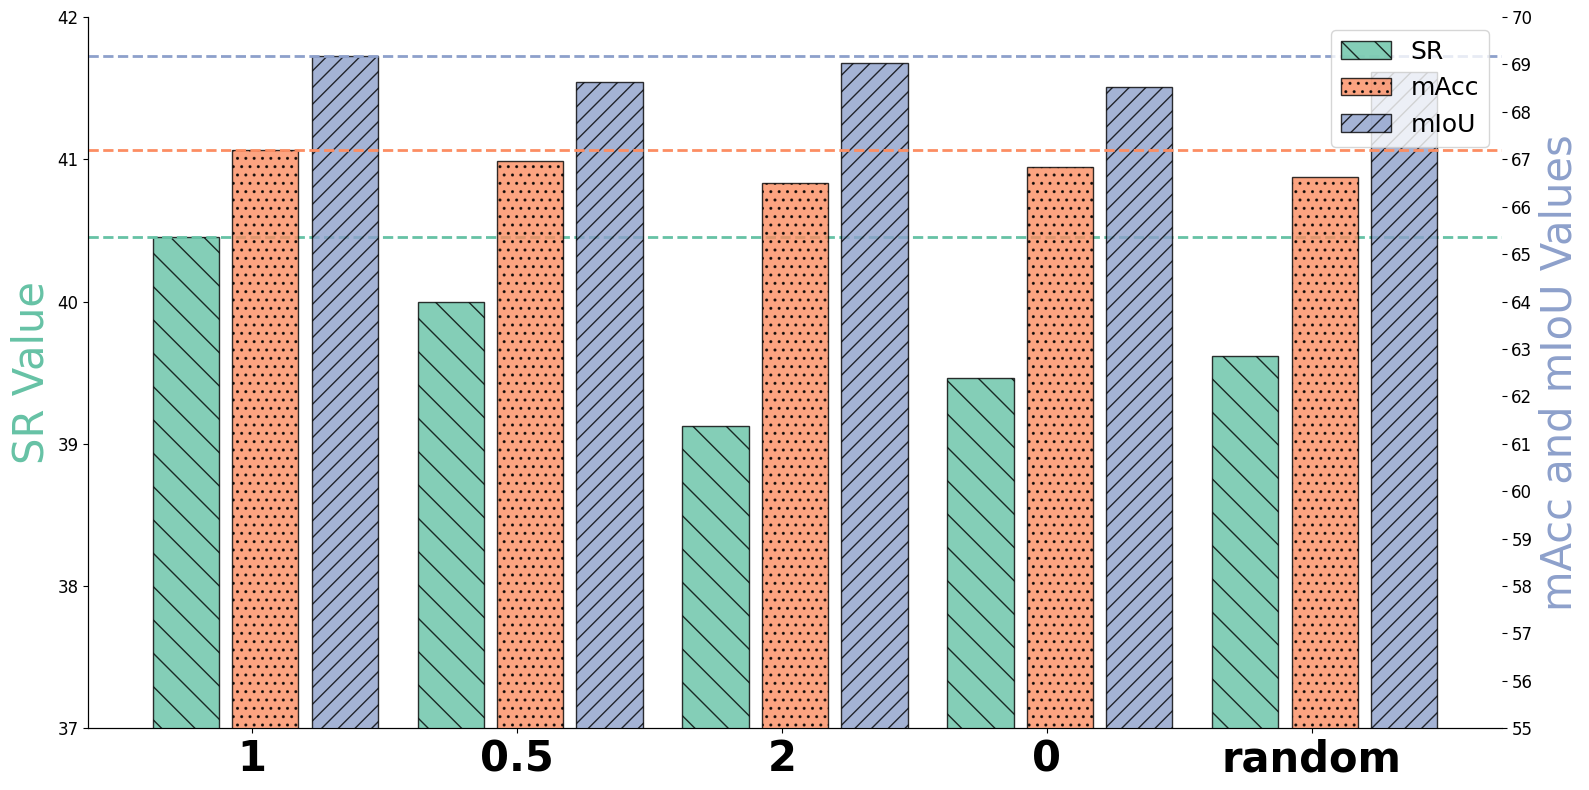
\includegraphics[width=0.45\textwidth]{figures/int1.png}
    \label{fig:int1}
}
\hfill
\subfloat[Ablation studies on different return values.]{%
    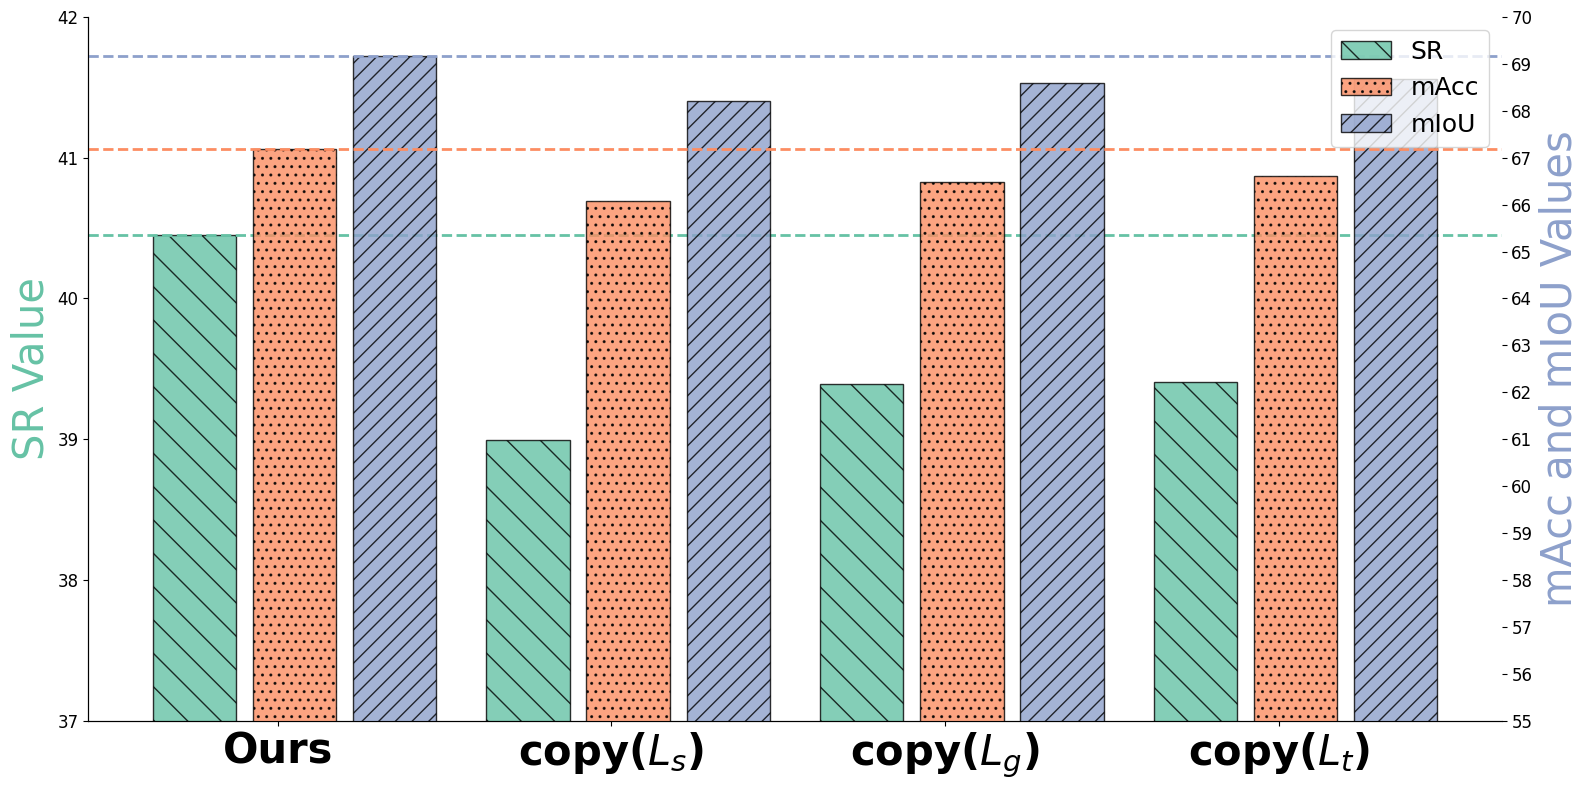
\includegraphics[width=0.45\textwidth]{figures/int2.png}
    \label{fig:int2}
}
\vfill
\subfloat[Ablation studies on selection with different interpolated features.]{
    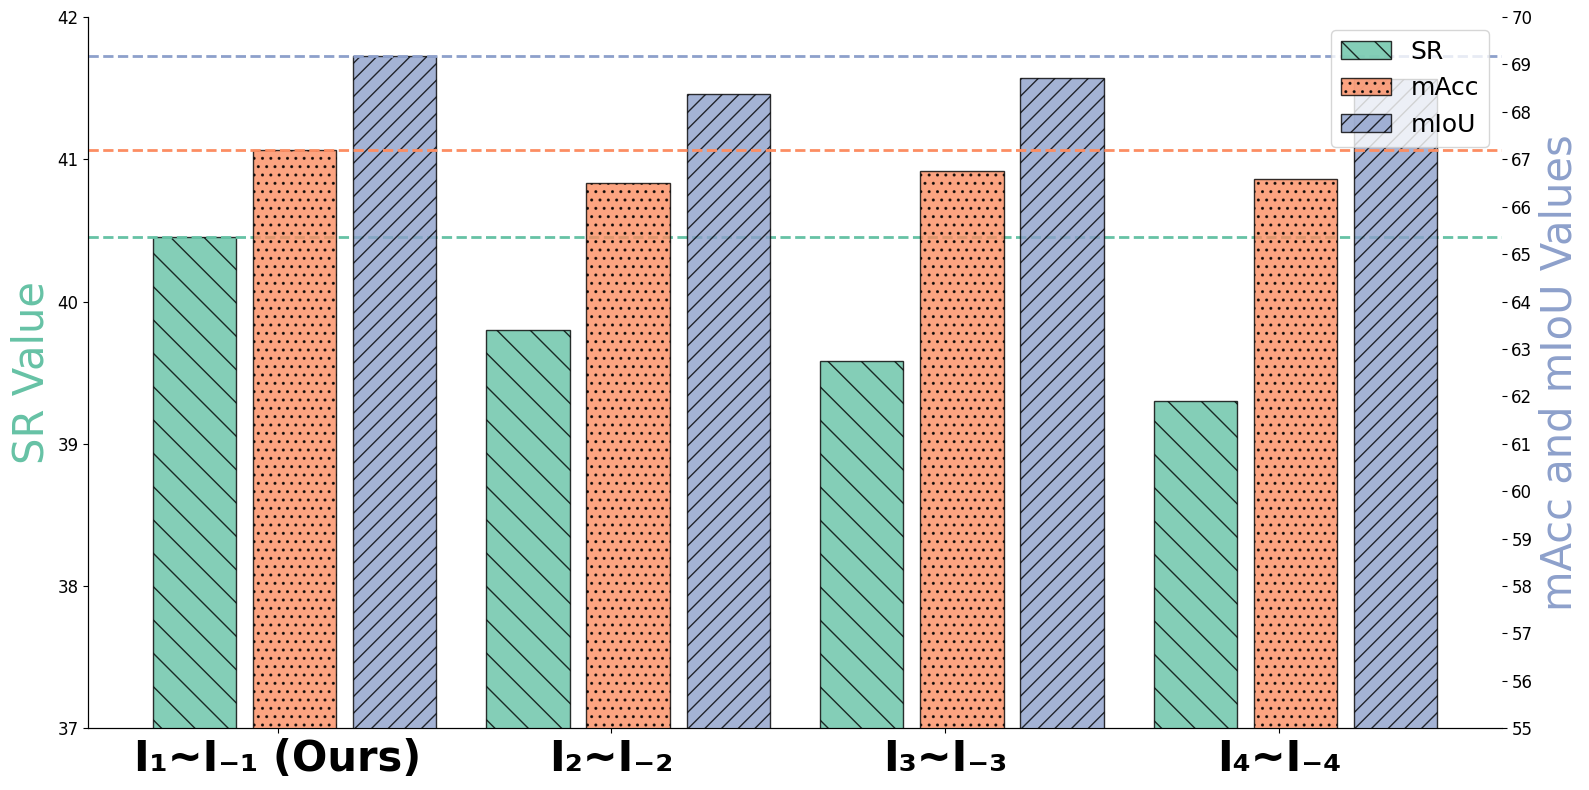
\includegraphics[width=0.45\textwidth]{figures/int3.png}
    \label{fig:int3}
}
\hfill
\subfloat[Ablation studies on different fusion methods.]{%
    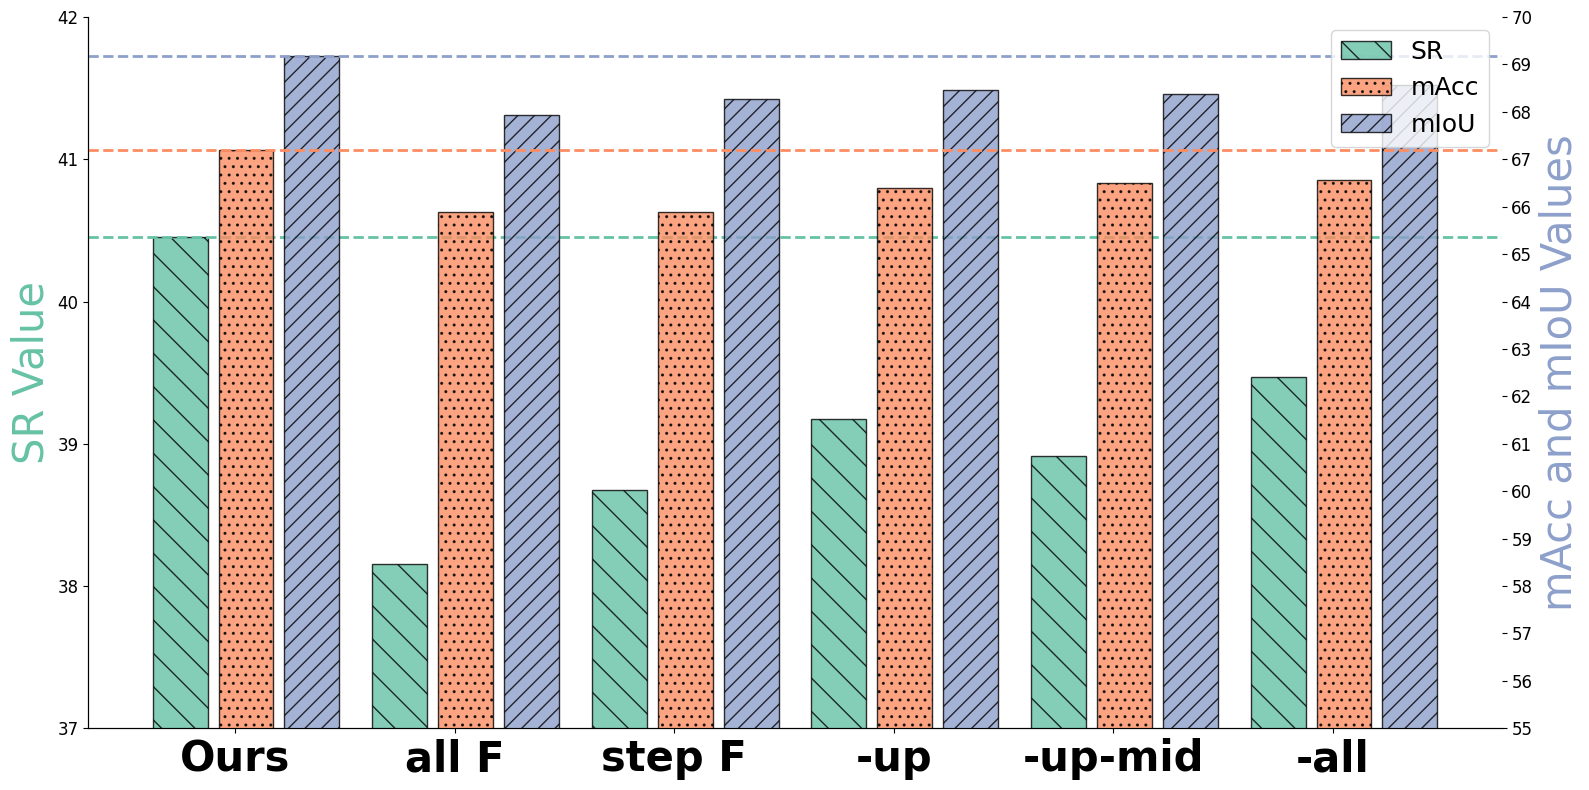
\includegraphics[width=0.45\textwidth]{figures/int4.png}
    \label{fig:int4}
}
\caption{Ablation Studies for Interpolation Strategy. \Cref{fig:int1} shows different initialization coefficient values $\tau$; \Cref{fig:int2} illustrates the features generated by the interpolator, where ``$copy(L_g)$'' means $I_j = L_g$, and ``$copy(L_t)$'' indicates $I_j = L_s$ for $j \leq \frac{M}{2}$ and $I_j = L_g$ for $j > \frac{M}{2}$. In \Cref{fig:int3}, $I_i$ to $I_{-i}$ indicates that we use interpolated features from the $i$-th to the last $i$-th for the second interpolation. In \Cref{fig:int4}, ``all F'' denotes that each cross-attention module receives $F_{1:M}$ as input, ``step F'' means we input one $F_{\frac{M}{2}}$ at the start and gradually increase the number of features inputted towards both sides, and ``-all'' indicates that we omit inputting $F_j$ during the upsampling, middle-sampling, and downsampling processes in U-Net. }
\label{fig:four_images2}
\end{figure}